\documentclass[12pt,a4paper]{article}

% --------------------
% Packages
% --------------------
\usepackage[margin=1in]{geometry}
\usepackage{graphicx}
\usepackage{fancyhdr}
\usepackage{setspace}
\usepackage{titlesec}
\usepackage{enumitem}
\usepackage{xcolor}
\usepackage{hyperref}
\usepackage{subcaption}
\usepackage[table]{xcolor}
\usepackage{colortbl}
\usepackage{booktabs}
\usepackage{makecell}
\usepackage{multirow}
\usepackage{svg}
\usepackage{amsmath}
\usepackage{amsfonts}
\usepackage{tikz}
\usetikzlibrary{calc}
\usetikzlibrary{positioning,arrows.meta,shapes.geometric}
\usetikzlibrary{positioning,calc,fit,backgrounds}

% --------------------
% Paragraph formatting
% --------------------
\setlength{\parindent}{0pt}  % Remove paragraph indentation
% \setlength{\parskip}{1em}    % Optional: add space between paragraphs

% --------------------
% Project Information
% --------------------
\newcommand{\CompanyName}{Pressure Control Solutions}
\newcommand{\ReportTitle}{Linear-Quadratic-Integral Control}
\newcommand{\ReportSubTitle}{System identification and model-based control of an EQ-DA}
\newcommand{\AuthorName}{Hubald Verzijl}
\newcommand{\AuthorEmail}{hubald@pressurecontrolsolutions.com}
\newcommand{\VersionNumber}{0.1}
\newcommand{\ReportDate}{\today}

\hypersetup{
    colorlinks=true,
    linkcolor=blue,
    filecolor=magenta,      
    urlcolor=cyan,
    pdftitle={\ReportTitle},
    pdfauthor={\AuthorName},
    pdfkeywords={Pressure, Dynamics, Quattroflow, Equilibar, Report},
}

% --------------------
% Header & Footer
% --------------------
\pagestyle{fancy}
\fancyhf{} % Clear default header/footer

% Header
\setlength{\headheight}{30pt}
\fancyhead[L]{%
  
\includegraphics[height=0.75cm]{../images/logo.png}
}
\fancyhead[R]{Report Version \VersionNumber}

% Footer
\fancyfoot[C]{\thepage}

\renewcommand{\headrulewidth}{0.4pt}
\renewcommand{\footrulewidth}{0.4pt}

% --------------------
% Title Page
% --------------------
\begin{document}

\begin{titlepage}
    \thispagestyle{fancy}
    \fancyfoot{} % Clear footer for this page only
    \centering
    \vspace*{2cm}
    {\Huge \bfseries \ReportTitle \par}
    \vspace{0.5cm}
    {\Large \ReportSubTitle \par}
    \vspace{2cm}
    % \begin{center}
        % \includegraphics[width=0.8\textwidth]{images/setup.pdf}
    % \end{center}
    \vspace{2cm}
    {\Large \CompanyName \par}
    \vspace{0.25cm}
    {\small Author: \AuthorName \par}
    \vspace{0.25cm}
    {\small Report Version: \VersionNumber \par}
    \vspace{0.25cm}
    {\small Date: \ReportDate \par}
    \vfill
\end{titlepage}

\section*{Introduction}
This document describes the design of a Linear-Quadratic-Integral (LQI) controller for the EQ-DA system. The LQI controller is designed based on a state-space model identified from closed-loop data collected using a PID controller with PRBS excitation. The identified model is used to design a Kalman state observer and an LQI controller that minimizes a cost function while ensuring zero steady-state error. This strategy can be used for the inner loop and the outer loop of the EQ-DA. The following sections describe the methods used for system identification, state estimation, and controller design, as well as the results obtained from experiments.

\tableofcontents
\newpage

\section{Methods}
Goal of this section is to explain the state-feedback controller design. Figure \ref{fig:workflow} shows the proposed method. The method consists of closed-loop data collection based on a closed-loop stable PID system, \texttt{n4sid} to detmermine the associated state-space model, Kalman state estimation setup, and LQI control design based on the identified model. The following sections describe each step in detail.

\begin{figure}[ht]
    \centering
    \resizebox{\textwidth}{!}{%
    \begin{tikzpicture}[
        auto,
        >=latex,
        node distance=1cm and 1cm,
        block/.style={
            draw,
            rounded corners,
            minimum width=3.6cm,
            minimum height=1.2cm,
              align=center
        }
    ]
        \node[block] (pid) {Closed-loop\\data collection \\(Based on PID with\\PRBS excitation)};
        \node[block, right=of pid] (n4sid) {State-space model\\i dentification\\(\texttt{n4sid})};
        \node[block, right=of n4sid] (kf) {Kalman state-space\\filter design};
        \node[block, right=of kf] (lqi) {LQR and LQI \\controller design};

        \draw[->] (pid) -- (n4sid);
        \draw[->] (n4sid) -- (kf);
        \draw[->] (kf) -- (lqi);
    \end{tikzpicture}
    }
    \caption{Workflow of the proposed control strategy.}
    \label{fig:workflow}
\end{figure}

\subsection{Control strategy}
Figure \ref{fig:control_architecture} shows the proposed control architecture, which consists of a Kalman state observer, an LQR controller, and an integrator to eliminate steady-state error. The Kalman state observer estimates the system states from the measured output and control input. The estimated states are fed back through the gain matrix $K$, while the tracking error is integrated to provide zero steady-state error. The LQR controller minimizes a cost function that balances state deviations and control effort. To eliminate steady-state error, the system is augmented with an integrator on the output error, resulting in a Linear Quadratic Integral (LQI) controller. The augmented state vector includes both the original states and the integrator state, allowing for improved tracking performance.
\begin{figure}[ht] 
\centering 
\begin{tikzpicture}[ 
  auto, node distance=1cm, >=latex, 
  block/.style={ 
    draw, rectangle, 
    minimum height=1.1cm, minimum width=2cm, align=center 
  }, 
  sum/.style={ 
    draw, circle, inner sep=0pt, minimum size=6mm 
  } 
]
  % Nodes 
  \node (r) {$r(k)$}; 
  \node [sum, right=1cm of r] (sum) {}; 
  \node at ($(sum.west)+(-0.25,-0.25)$) {\scriptsize $+$}; 
  \node at ($(sum.south)+(-0.25,-0.25)$) {\scriptsize $-$}; 
  \node [block, right=1cm of sum] (pid) {Integrator}; 
  \node [sum, right=2cm of pid] (u) {}; 
  \node at ($(u.west)+(-0.25,-0.25)$) {\scriptsize $+$}; 
  \node at ($(u.south)+(-0.25,-0.25)$) {\scriptsize $+$}; 
  \node [block, right=2cm of u] (plant) {EQ-DA}; 
  \coordinate[right=1cm of plant] (output); 
  \node [block, below=1cm of plant] (kalman) {Kalman\\Observer}; 
  \node [block, below=1.25cm of u] (gain) {$-K$}; 


  % LQI background box   
  \begin{pgfonlayer}{background} 
    \node[ draw=red!60, fill=red!5, rounded corners, inner xsep=20pt, inner ysep=30pt, 
           fit=(sum) (kalman), label=below:\textcolor{red}{\textbf{LQI} } ] {}; 
  \end{pgfonlayer} 
    
% LQR with state feedback background box
  \begin{pgfonlayer}{background} 
    \node[ draw=blue!60, fill=blue!10, rounded corners, inner sep=10pt, 
           fit=(kalman) (u) (gain), label=above:{\textcolor{blue}{\textbf{LQR with state feedback}} } ] {}; 
  \end{pgfonlayer} 

  % Main loop 
  \draw[->] (r) -- (sum); 
  \draw[->] (sum) -- node[above] {$e(k)$} (pid); 
  \draw[->] (pid) -- (u); 
  \draw[->] (u) -- node[above] {$u(k)$} (plant); 
  \draw[-] (plant.east) -- (output); 
  \draw[->] (output) -- ++(1,0) node[right] {$y(k)$}; 
  
  % Kalman observer inputs 
  \draw[->] (output) |- ($(kalman.east)+(0,+0.25)$);
  \draw[->] ($(u.east)+(1,0)$) |- ($(kalman.west)-(0,-0.25)$); 
  \draw[dashdotted,->] ($(kalman.east)+(0,-0.25)$) -- ($(kalman.east)+(2,-0.25)$) node[right] {$\hat{y}(k)$};
  
  % State feedback 
  \draw[->] ($(kalman.west)+(0,-0.25)$) -- node[below] {$\hat{x}(k)$} ($(gain.east)+(0,-0.25)$); 
  \draw[->] (gain) -- (u); 
  
  % Output feedback to integrator 
  \draw[->] (output) -- ($(output)-(0,3.25)$) -| (sum.south); 
\end{tikzpicture} 

\caption{LQI control architecture with Kalman state observer. The observer estimates the system states from the measured output and control input. The estimated states are fed back through the gain matrix $K$, while the tracking error is integrated to provide zero steady-state error.} 
\label{fig:control_architecture} 
\end{figure}

\newpage
\subsection{State-space model}
One of the most important tasks in control system design is the creation of a state-space model resenting the EQ-DA. The state-space model is a mathematical representation of the system dynamics in terms of state variables, inputs, and outputs. The state-space representation is given by:
\begin{equation}
\begin{aligned}
x[k+1] &= Ax[k] + Bu[k] \\
y[k] &= Cx[k] + Du[k]
\end{aligned}
\end{equation}
where:
\begin{itemize}
    \item $k$ is the discrete time index,
    \item $x[k] \in \mathbb{R}^{n}$ is the state vector, the amount of states depends on the order of the system,
    \item $u[k] \in \mathbb{R}^{m}$ is the control input, $m$ is the amount of inputs of the system,
    \item $y[k] \in \mathbb{R}^{p}$ is the output, $p$ is the amount of outputs of the system,
    \item $A \in \mathbb{R}^{n \times n}$, $B \in \mathbb{R}^{n \times m}$, $C \in \mathbb{R}^{p \times n}$, and $D \in \mathbb{R}^{p \times m}$ are the system matrices.
\end{itemize}
A dynamically complex system results in a higher order state-space model (higher $n$), while a simpler system results in a lower order state-space model (lower $n$). The state-space model can be used to design controllers, such as LQR and LQI controllers, to achieve desired performance and stability characteristics. Model predictive control (MPC) can also be designed based on the state-space model, allowing for optimal control of the system over a finite time horizon.

\subsection{State-space model identification}
As the EQ-DA is open-loop unstable, closed-loop identification is used to obtain its state-space model. Figure \ref{fig:closedloop_identification} shows a roughly tuned PID controller to stabilize the system during identification, while a pseudo-random binary sequence (PRBS) excites it across a range of frequencies. The PRBS is generated using the \texttt{prbs} function from the \texttt{python-control} package and applied as the reference input. The resulting input-output data is then used with the \texttt{n4sid} method to estimate the state-space matrices $A$, $B$, $C$, and $D$. Importantly, the PID output acts as the input to the EQ-DA system and therefore as the input to \texttt{n4sid}. The identified model can subsequently be used for controller design and analysis. 

\begin{figure}[ht] \centering \begin{tikzpicture}[ auto, node distance=1cm, >=latex, 
    block/.style={draw, rectangle, minimum height=1cm, minimum width=2cm}, 
    sum/.style={draw, circle, inner sep=0pt, minimum size=6mm}, ] 
% Nodes 
\node (r) {PRBS $r(k)$}; 
\node [sum, right=1cm of r] (sum) {}; 
\node at ($(sum.west)+(-0.25,-0.25)$) {\scriptsize $+$};
 \node at ($(sum.south)+(-0.25,-0.25)$) {\scriptsize $-$};
\node [block, right=1cm of sum] (pid) {PID}; 
\coordinate[right=0.5cm of pid] (u);
\node [block, right=0.5cm of u] (plant) {EQ-DA}; 
\coordinate[right=0.5cm of plant] (output);
\node [below=1.5cm of output] (y_n4sid) {$y(k)$}; 
\node [block, below=2cm of plant] (n4sid) {\texttt{n4sid}}; 
\coordinate[below=1cm of sum] (fb);
\node [below=1.5cm of u] (u_n4sid) {$u(k)$}; 


% Connections 
\draw[->] (r) -- (sum); 
\draw[->] (sum) -- node {$e(k)$} (pid); 
\draw[->] (pid) -- node[above] {$u(k)$} (plant);
\draw[->] (output) -- ++(1,0) node[right] {$y(k)$}; 

% Feedback 
\draw[->] (plant.east) -- (output) -- ++(0,-1) -- ($(sum)+(0,-1)$) -- (sum.south);

% Signals to identification 
\draw[dashdotted] (u) -- (u_n4sid);
\draw[dashdotted,->] (u_n4sid) |- (n4sid.west); 
\draw[dashdotted] ($(output)+(0,-1)$) -- ++(0,-0.5); 
\draw[dashdotted,->] (y_n4sid) |- (n4sid.east);

% Output of identification 
\draw[->] (n4sid.south) -- ++(0,-0.5) node[below, align=center] {Estimated state-space model\\$\{A,B,C,D\}$}; 
\end{tikzpicture} 
\caption{Closed-loop system identification of the EQ-DA system. A PRBS reference excites the closed-loop system while a PID controller stabilizes the otherwise open-loop unstable plant. The controller output $u(k)$ and measured output $y(k)$ are used by the \texttt{n4sid} algorithm to estimate the state-space matrices $A$, $B$, $C$, and $D$.} 
\label{fig:closedloop_identification} 
\end{figure}

\newpage
\subsection{Kalman observer}
Different types of state observers can be designed. In this report, a Kalman state observer is designed based on the identified state-space model. The Kalman filter is an optimal state estimator that minimizes the estimation error covariance by considering both the process noise and measurement noise. Ideally, $\hat{y}(k)$ will be equal to $y(k)$ from Figure \ref{fig:control_architecture}, but in practice, they converge to the true values, but there will be some estimation error. The Kalman filter equations are given by:
\begin{equation}
\begin{aligned}
\hat{x}[k+1] &= A \hat{x}[k] + B u[k] + L (y[k] - \hat{y}[k]) \\
\hat{y}[k] &= C \hat{x}[k] + D u[k]
\end{aligned}
\end{equation}
where $L$ is the Kalman gain matrix, which is computed by solving the discrete-time algebraic Riccati equation. The Kalman gain $L$ determines how much weight is given to the measurement error in updating the state estimate. The Kalman filter provides an optimal estimate of the system states, which can be used for feedback control in the LQR and LQI controllers.


\newpage
\subsection{State-feedback controller design}
\subsubsection{LQR control}
First, a Linear Quadratic Regulator (LQR) controller is designed based on the identified state-space model. The LQR controllaw is given by 
\begin{equation}
u[k] = -K x[k]
\end{equation}
where $K$ is the gain matrix obtained by solving the discrete-time algebraic Riccati equation. The Ricatti equation is solved using the \texttt{dlqr} function from the \texttt{python-control} package, which computes the optimal gain matrix $K$ that minimizes the cost function:
\begin{equation}
J = \sum_{k=0}^{\infty} (x[k]^T Q x[k] + u[k]^T R u[k])
\end{equation}
where $Q$ and $R$ are weighting matrices that penalize deviations from the desired state and control effort, respectively. These can be chosen based on a slider tool and changes the behavior from conservative to aggressive. After solving, the optimal control law is given by:
\begin{equation}
u[k] = -K x[k].
\end{equation}
However, the LQR controller does not guarantee zero steady-state error for tracking a reference signal. To address this, an error integrator is added to the system, in the form of 
\begin{equation}
z[k+1] = z[k] + T_s\left(r[k] - y[k]\right)
\end{equation}
where $T_s$ is the sampling time, $r[k]$ is the reference signal, and $y[k]$ is the output. The integrator state $z[k]$ accumulates the error between the reference and the output, allowing the controller to adjust the control input to eliminate steady-state error, resulting in an LQI controller. 


\subsubsection{LQI control}
The LQI controller augments the state-space model with an integrator on the output error. The augmented state vector is defined as:
\begin{equation}
\tilde{x}[k] = \begin{bmatrix} x[k] \\ z[k] \end{bmatrix}
\end{equation}
where $z[k]$ is the integrator state, which accumulates the error between the reference signal and the output. The augmented system dynamics are given by:
\begin{equation}
\begin{aligned}
\tilde{x}[k+1] &= \tilde{A} \tilde{x}[k] + \tilde{B} u[k] + \tilde{E} r[k] \\
y[k] &= \tilde{C} \tilde{x}[k] + \tilde{D} u[k]
\end{aligned}
\end{equation}
where:
\begin{equation}
\tilde{A} = \begin{bmatrix} A & 0 \\ -C \cdot T_s & I \end{bmatrix}, \quad
\tilde{B} = \begin{bmatrix} B \\ -D \cdot T_s \end{bmatrix}, \quad
\tilde{C} = \begin{bmatrix} C & 0 \end{bmatrix}, \quad
\tilde{D} = D, \quad
\tilde{E} = \begin{bmatrix} 0 \\ T_s \end{bmatrix}
\end{equation}
The controllaw for the LQI controller is given by:
\begin{equation}
u[k] = -\tilde{K} \tilde{x}[k].
\end{equation}
The LQI controller is designed by defining again a cost function, but now for the augmented system:
\begin{equation}
J = \sum_{k=0}^{\infty} (\tilde{x}[k]^T \tilde{Q}_{LQI} \tilde{x}[k] + u[k]^T \tilde{R}_{LQI} u[k])
\end{equation}
where 
\begin{equation}
\tilde{Q}_{LQI} = \begin{bmatrix} Q & 0 \\ 0 & q_i \end{bmatrix}, \quad
\tilde{R}_{LQI} = R.
\end{equation}
Parameter $q_i$ is the weight on the integrator state, which can be slider-tuned to achieve the desired trade-off between tracking performance and control effort. To 





\newpage
\section{Results: internal loop}

\section{Results: external loop}

\newpage
\section*{Version control}
\addcontentsline{toc}{section}{Version control}

\begin{tabular}{|c|c|c|}
\hline
Version & Date & Description \\
\hline
0.1 & August 21, 2026 & Initial draft \\
\hline
\end{tabular}

\end{document}